\documentclass[dvipdfmx,11pt]{beamer}

\usetheme{Madrid}
\usefonttheme{professionalfonts}

\definecolor{tohokuPurple}{RGB}{62,21,134}
\setbeamercolor{structure}{fg=tohokuPurple}
\setbeamercolor{frametitle}{bg=tohokuPurple, fg=white}

\setbeamercolor{title}{fg=white, bg=tohokuPurple}
\setbeamercolor{author}{fg=black}
\setbeamercolor{institute}{fg=black}
\setbeamercolor{date}{fg=black}

\setbeamercolor{block title}{bg=tohokuPurple, fg=white}
\setbeamercolor{block body}{bg=tohokuPurple!5, fg=black}
\setbeamertemplate{navigation symbols}{}

\usepackage{amsmath,amssymb,bm}
\usepackage{listings,booktabs}
\usepackage{graphicx}
\graphicspath{{../figures/}{figures/}}
\usepackage{tikz}
\usetikzlibrary{arrows.meta,positioning}
\usepackage{hyperref}
\usepackage{bookmark}

\title[GSE-VAR]{GSE-VAR：解釈可能な深層VAR}
\subtitle{Gated Self-Explaining Vector Autoregression}
\author[栗田 煌矢]{
  東北大学経済学部4年李研\texorpdfstring{\\}{ }\
  栗田 煌矢}

\date{\today}

\begin{document}

\begin{frame}
  \titlepage
\end{frame}


\begin{frame}{VAR(ベクトル自己回帰)}



VAR(ベクトル自己回帰)モデルは、目的変数がベクトルであり、それを過去の変数ベクトルに回帰する。

\vspace{0.5em}

線形VARなら、
  \[
    x_t
    =
    \sum_{k=1}^{K}
    \Phi_k x_{t-k}
    +
    \varepsilon_t
  \]

$\Phi_k$はラグ$k$に対応する係数行列。

VARをベースとしたグレンジャー因果推定モデルがテーマとなる。



\end{frame}



\begin{frame}{GSE-VARについて}

  \begin{enumerate}
    \item 係数生成ネットで状態依存的かつ符号解釈が可能な係数を学習する。
    \item 構造的正則化により、係数行列をまとめてスパース化する。
    \item 学習可能な非負の\texttt{causal\_gate}を用い、これを近接勾配法で厳密にゼロ化することで、閾値なしでグレンジャー因果行列を得る。
  \end{enumerate}

\end{frame}

\begin{frame}{GSE-VARの貢献}
  \small
  GSE-VARに関して、次を同時に満たす点が貢献であると考える。

  \vspace{0.4em}
  \begin{enumerate}
    \item \textbf{非線形・状態依存性}：時点ごとに変化する非線形効果を表現できる。
    \item \textbf{厳密なスパース性}：存在しない変数間関係を厳密なゼロとしてまとめて除去。
    \item \textbf{係数としての解釈性}：変数・ラグごとに効果の方向と大きさを読み取れる。
  \end{enumerate}

  \vspace{0.5em}
  \scriptsize
  \setlength{\tabcolsep}{4pt}
  \renewcommand{\arraystretch}{1.25}
  \center
  \begin{tabular}{@{}lccc@{}}
    \toprule
    手法 & 非線形・状態依存 & 厳密なスパース性 & 係数の解釈 \\
    \midrule
    線形VAR & × & × & ○ \\
    eSRU & △ & ○ & × \\
    NGC & △ & ○ & ×\\
    GVAR & ○ & × & ○ \\
    \textbf{GSE-VAR} & \textbf{○} & \textbf{○} & \textbf{○} \\
    \bottomrule
  \end{tabular}

  \vspace{0.6em}
  \normalsize
\textbf{三つの特徴を全て満たすことで新規性を出す。}
\end{frame}


\begin{frame}{背景：GVARとNeural Granger Causality}
  GSE-VARは、次の2つの既存手法をcausal gateで統合している。

  \begin{enumerate}
    \item GVAR：状態依存的で符号解釈が可能な係数行列をニューラルネットワークで生成する(Marcinkevičs, R., \& Vogt, J. E.,2021)。
    \item Neural-GC：ニューラルネットワークに構造的スパース性を導入し、Granger因果性を推定する(Tank et al.,2021)。
  \end{enumerate}

  \vspace{0.5em}

  \[
    \texttt{causal\_gate.shape} = [\text{lag}, \text{target}, \text{source}],
    \qquad
    G_{k,i,j}\geq 0
  \]

\end{frame}

\begin{frame}{GSE-VARの全体像}
\centering
\small
\resizebox{0.98\linewidth}{!}{%
\begin{tikzpicture}[
  node distance=0.75cm and 0.8cm,
  box/.style={draw, rounded corners, align=center, minimum width=2.45cm, minimum height=0.8cm},
  gate/.style={draw, rounded corners, align=center, minimum width=2.45cm, minimum height=0.8cm, fill=blue!8},
  op/.style={draw, circle, inner sep=1.5pt},
  sumop/.style={draw, circle, inner sep=2pt, fill=gray!8},
  arr/.style={-Latex, thick}
]
  \node[box] (input) {ラグ入力\\$x_{t-k}$};
  \node[op, right=of input] (inprod) {$\odot$};
  \node[box, right=of inprod] (coefnet) {係数出力ネット};
  \node[box, right=of coefnet] (phi) {状態依存係数\\$\Phi_{k,i,:}(u_{k,i,t})$};
  \node[gate, below=of phi] (gate) {causal gate\\$G_{k,i,:}\geq0$};
  \node[op, right=of phi] (prod) {$\odot$};
  \node[box, right=of prod] (eff) {有効係数\\$\tilde{\Phi}_{k,i,:}$};
  \node[op, right=of eff] (mprod) {$\times$};
  \node[box, right=of mprod] (pred) {予測値\\$\hat{x}_{i,t}$};

  \draw[arr] (input) -- (inprod);
  \draw[arr] (gate.west) -| (inprod);
  \draw[arr] (inprod) -- (coefnet);
  \draw[arr] (coefnet) -- (phi);
  \draw[arr] (phi) -- (prod);
  \draw[arr] (gate) -| (prod);
  \draw[arr] (prod) -- (eff);
  \draw[arr] (eff) -- (mprod);
  \draw[arr] (input.north) to[out=70,in=115,looseness=0.35] (mprod.north);
  \draw[arr] (mprod) -- (pred);

  \node[align=center, below=0.25cm of gate] {\scriptsize 近接勾配法で\\[-0.1em]\scriptsize 厳密ゼロ化};
\end{tikzpicture}
}

\vspace{0.6em}
\[
  u_{k,i,t}=G_{k,i,:}\odot x_{t-k},
  \qquad
  \tilde{\Phi}_{k,i,:}
  =
  G_{k,i,:}\odot \Phi_{k,i,:}(u_{k,i,t})
\]
\[
  \hat{x}_{i,t}
  =
  \sum_{k=1}^{K}
  \tilde{\Phi}_{k,i,:}x_{t-k}
\]
\end{frame}

\begin{frame}{GVAR(Marcinkevičs, R., \& Vogt, J. E.,2021)}
  $p$変量時系列を
  \[
    x_t = (x_{t,1}, \ldots, x_{t,p})^\top \in \mathbb{R}^{p}
  \]
  とする。自己回帰次数を$K$とすると、一般化VAR(GVAR)は次のように表される。

  \[
    x_t
    =
    \sum_{k=1}^{K}
    \Phi_{k(x_{t-k})} x_{t-k}
    +
    \varepsilon_t
  \]

  $\Phi_{k(x_{t-k})} \in \mathbb{R}^{p \times p}$はラグ$k$に対応する
  \textbf{状態依存的}な係数行列であり、これがニューラルネットの出力となる。

  \vspace{1.0em}
  \begin{center}
    \textbf{特徴}：係数の符号解釈が可能であるが、事後的な閾値処理が必要。
  \end{center}


\end{frame}


\begin{frame}{Neural Granger Causality (NGC) (Tank et al.,2021)}

  NNのスパース制約を工夫し、Granger因果性を推定する手法である。

  \vspace{0.5em}
  \begin{block}{Theorem (Tank et al.,2021)}
    変数$j$が変数$i$をGranger causeしないための十分条件は、
    すべてのラグにおいて$j$から$i$への重みがゼロであることである。
  \end{block}
  この条件を満たすように、\textbf{入力層重みに対して構造的な厳密スパース最適化(近接勾配法)}を行う。

  \vspace{1.0em}

  \begin{center}
    \textbf{特徴}：厳密なスパース性により、閾値処理無しかつグレンジャー非因果性が保証。係数の符号は意味を持たない。
  \end{center}
\end{frame}

\begin{frame}{Causal GateによるGVARとNGCの統合}
  両者の統合をしたい。
  \begin{block}{グレンジャー非因果性保証の課題}
    GVARにおいて、係数はNNで生成するため、あるsource変数$x_j$は、自身の係数だけでなく、
    他のsourceに対応する係数の生成にも影響する。
  \end{block}


  \vspace{0.5em}
  そこで、target変数ごとにラグ別の係数生成NN(=$pK$個のNN)を用い、NNへの入力と生成後の係数に\textbf{入力値に依存しない}\texttt{causal\_gate}を適用する。
  \[
    u_{k,i,t}=G_{k,i,:}\odot x_{t-k}
  \]

  \[
    \tilde{\Phi}_{k,i,:}
    =
    G_{k,i,:}\odot \Phi_{k,i,:}(u_{k,i,t})
  \]

  \vspace{0.3em}
  これにより、$G_{k,i,j}=0$なら、$x_{j,t-k}$から$x_{it}$への効果がゼロになることが保証される。
\end{frame}

\begin{frame}{本研究のGranger非因果性の定義}
  変数$x_j$が変数$x_i$をGranger causeしないための十分条件は、
  すべてのラグにおいて$x_j$から$x_i$への効果がゼロであることである。
  つまり、
  \[
    G_{1,i,j} = G_{2,i,j} = \cdots = G_{K,i,j} = 0
  \]

  このとき、すべてのラグについて$x_j$は、

  \begin{enumerate}
    \item 有効係数を$x_{j,t-k}$に直接乗じる経路
    \item target $i$の係数生成ネットワークへの入力経路
  \end{enumerate}

  の両方から除外される。

非因果性を主張するために、gateの値を厳密な0にする工夫が必要。
\end{frame}

\begin{frame}{Causal Gateの補足}
1. 解釈上のメリット
\begin{itemize}
  \item (Granger因果の静的なスケルトンだけ$G_k$が制御し、その強弱は$\Phi_{k,i,:}(u_{k,i,t})$が表現するという役割の分離。)
  \item gateに着目するだけで変数が推論に使われてるか解釈できる。
\end{itemize}

2. Granger非因果性を保証するための都合
\begin{enumerate}
  \item ある変数が係数生成ネットの入力に使われなくても、線形結合の段階で使ってしまう。
  \item ある変数に関するgateの値が0になっても、他の変数のgateを通じてtargetの予測に寄与してしまう。
  \item 二カ所にgate作用することで、gateが0ならGranger非因果を担保する。
\end{enumerate}

\end{frame}




\begin{frame}{目的関数}
  予測損失、時間方向の平滑化、NGC正則化からなる。

  \[
    \mathcal{L}
    =
    \mathcal{L}_{\mathrm{pred}}
    +
    \mathcal{R}_{\mathrm{smooth}}
    +
    \mathcal{R}_{\mathrm{ngc}}
  \]

  \vspace{0.3em}

  予測損失は平均二乗誤差である。

  \[
    \mathcal{L}_{\mathrm{pred}}
    =
    \frac{1}{N}
    \sum_t
    \left\|
      x_t - \hat{x}_t
    \right\|_2^2
  \]

\end{frame}


\begin{frame}{Temporal Smoothness}
  状態依存係数を用いるため、係数が過度に振動しないための平滑化ペナルティ；

  \[
    \mathcal{R}_{\mathrm{smooth}}
    =
    \frac{\lambda_{\mathrm{smooth}}}{|\mathcal{T}|}
    \sum_{t \in \mathcal{T}}
    \left\|
      \tilde{\Phi}_{t+1}
      -
      \tilde{\Phi}_t
    \right\|_F^2
  \]

 隣接する時点間で係数の値(or 符号)が過度に変わるという
 不自然な動きを抑制し、過学習防止や解釈の妥当性を実現する。
\end{frame}

\begin{frame}{NGC型正則化：Sparse Group Lasso}
  \small
  Sparse Group Lassoは、特定の変数のエッジをすべてのラグでまとめて0にする圧力と、特定のラグの特定の変数のエッジを0にする圧力の両方を与える。

  \vspace{0.3em}
  \centering
  \resizebox{0.85\linewidth}{!}{%
  \begin{tikzpicture}[
    cell/.style={draw, rounded corners, minimum width=1.45cm, minimum height=0.72cm, align=center, fill=blue!8},
    note/.style={align=center},
    arr/.style={-Latex, thick}
  ]
    \node[note] at (-1.4,0) {edge\\$j \to i$};
    \node[cell] (g1) at (0.7,0) {$G_{1,i,j}$};
    \node[cell] (g2) at (2.25,0) {$G_{2,i,j}$};
    \node[cell] (dots) at (3.8,0) {$\cdots$};
    \node[cell] (gk) at (5.35,0) {$G_{K,i,j}$};

    \draw[very thick, blue!70!black] (-0.1,0.6) -- (6.15,0.6);
    \node[note, text=blue!70!black] at (3.0,1.05)
      {\scriptsize group lasso：edge全体をまとめて縮小};
    \draw[arr, blue!70!black] (3.0,0.9) -- (3.0,0.63);

    \foreach \x in {0.7,2.25,5.35} {
      \draw[arr, red!70!black] (\x,-0.75) -- (\x,-0.39);
    }
    \node[note, text=red!70!black] at (3.0,-1.1)
      {\scriptsize lasso：各lagのgateを個別に縮小};
  \end{tikzpicture}
  }

  \vspace{0.4em}
  \[
    \mathcal{R}_{\mathrm{SGL}}(G)
    =
    \lambda_{\mathrm{group}}
    \sum_{i,j}\|G_{:,i,j}\|_2
    +
    \lambda_{\mathrm{sparse}}
    \sum_{k,i,j}|G_{k,i,j}|
  \]
  \vspace{-0.4em}
  \scriptsize
  第1項はedge単位の削除、第2項はlag単位の削除を促す。
\end{frame}

\begin{frame}{NGC型正則化：Hierarchical Group Lasso}
  \small
  Hierarchical Group Lassoは古いラグに対応するgateの要素を
  優先的にゼロにする圧力をかけ、ラグの自動選択を実現する。

  \vspace{0.3em}
  \centering
  \resizebox{0.86\linewidth}{!}{%
  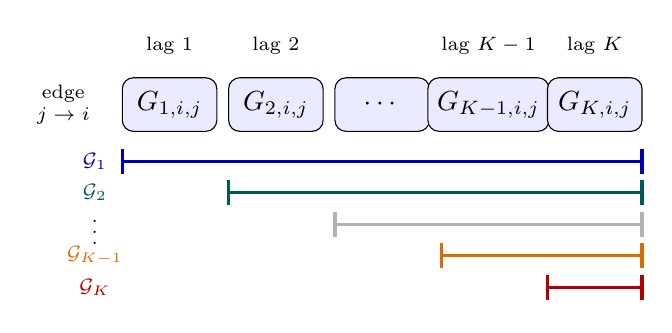
\begin{tikzpicture}[
    cell/.style={draw, rounded corners, minimum width=1.2cm, minimum height=0.68cm, align=center, fill=blue!8},
    note/.style={align=center, font=\scriptsize},
    brace/.style={very thick},
  ]
    \node[note] at (-1.35,0) {edge\\$j \to i$};
    \node[cell] (g1) at (0,0) {$G_{1,i,j}$};
    \node[cell] (g2) at (1.35,0) {$G_{2,i,j}$};
    \node[cell] (dots) at (2.7,0) {$\cdots$};
    \node[cell] (gkm) at (4.05,0) {$G_{K-1,i,j}$};
    \node[cell] (gk) at (5.4,0) {$G_{K,i,j}$};

    \node[font=\scriptsize] at (0,0.75) {lag 1};
    \node[font=\scriptsize] at (1.35,0.75) {lag 2};
    \node[font=\scriptsize] at (4.05,0.75) {lag $K-1$};
    \node[font=\scriptsize] at (5.4,0.75) {lag $K$};

    \node[note, text=blue!70!black] at (-0.95,-0.72) {$\mathcal{G}_{1}$};
    \draw[brace, blue!70!black] (-0.6,-0.72) -- (6.0,-0.72);
    \draw[brace, blue!70!black] (-0.6,-0.56) -- (-0.6,-0.88);
    \draw[brace, blue!70!black] (6.0,-0.56) -- (6.0,-0.88);

    \node[note, text=teal!70!black] at (-0.95,-1.12) {$\mathcal{G}_{2}$};
    \draw[brace, teal!70!black] (0.75,-1.12) -- (6.0,-1.12);
    \draw[brace, teal!70!black] (0.75,-0.96) -- (0.75,-1.28);
    \draw[brace, teal!70!black] (6.0,-0.96) -- (6.0,-1.28);

    \node[note] at (-0.95,-1.52) {$\vdots$};
    \draw[brace, gray!60] (2.1,-1.52) -- (6.0,-1.52);
    \draw[brace, gray!60] (2.1,-1.36) -- (2.1,-1.68);
    \draw[brace, gray!60] (6.0,-1.36) -- (6.0,-1.68);

    \node[note, text=orange!85!black] at (-0.95,-1.92) {$\mathcal{G}_{K-1}$};
    \draw[brace, orange!85!black] (3.45,-1.92) -- (6.0,-1.92);
    \draw[brace, orange!85!black] (3.45,-1.76) -- (3.45,-2.08);
    \draw[brace, orange!85!black] (6.0,-1.76) -- (6.0,-2.08);

    \node[note, text=red!70!black] at (-0.95,-2.32) {$\mathcal{G}_{K}$};
    \draw[brace, red!70!black] (4.8,-2.32) -- (6.0,-2.32);
    \draw[brace, red!70!black] (4.8,-2.16) -- (4.8,-2.48);
    \draw[brace, red!70!black] (6.0,-2.16) -- (6.0,-2.48);
  \end{tikzpicture}
  }

  \vspace{0.25em}
  \[
    \mathcal{G}_{k,i,j}
    =
    (G_{k,i,j},\ldots,G_{K,i,j}),
    \qquad
    \mathcal{R}_{\mathrm{HGL}}(G)
    =
    \lambda_{\mathrm{ngc}}
    \sum_{i,j}
    \sum_{k=1}^{K}
    \|\mathcal{G}_{k,i,j}\|_2
  \]

  \scriptsize

\end{frame}

\begin{frame}{Optimizer；近接勾配法(ISTA)}
ISTAは正則化で0に近づいたパラメータを、厳密に0にするための手法である。
ISTAでは次の2段階で\texttt{causal\_gate}を更新する。
\begin{center}
  \begin{enumerate}
    \item 予測損失と平滑化項に通常の勾配更新
    \item 更新後のgateを非負近接更新
  \end{enumerate}
\end{center}

  \[
    \text{勾配更新}
    \quad \longrightarrow \quad
    \text{非負近接更新}
    \quad \longrightarrow \quad
    G_{k,i,j}=0
  \]

  \vspace{0.6em}
  ここで使う超パラメータは、
  \[
    \eta \lambda
  \]
  であり、\textbf{モデルのパラメータ自体を0にする収縮圧力の強さ}をあらわす。

  \vspace{0.4em}
  全てのラグであるgateの値が0になれば...

\end{frame}

\begin{frame}{事後的な閾値処理との違い}

  \vspace{0.55em}
  \begin{block}{比較}
    \begin{itemize}
      \item 近接勾配法でgateが厳密に0になった変数は、係数項と係数生成ネットワークへの入力経路の両方から除外される。
      \item 事後的な閾値処理では、小さい非ゼロgateの変数が推論過程に使われる。
    \end{itemize}
  \end{block}
  \vspace{1.5em}
   事後的な閾値処理でGranger非因果性を主張しても、モデル学習には微小に使われてしまっていることになるため
   近接勾配法などで学習中に厳密に0にすることが望ましい。

\end{frame}


\begin{frame}{解釈}
  \small
  \begin{block}{学習後の解釈}
    \begin{enumerate}
      \item causal gateからのGranger因果行列$\hat{A}$
      \item 有効係数$\tilde{\Phi}_{k,t}$
    \end{enumerate}
  \end{block}
  \vspace{0.2em}
  \centering
  \resizebox{0.96\linewidth}{!}{%
  \begin{tikzpicture}[
    cell/.style={draw, minimum size=0.62cm, inner sep=0pt, align=center, font=\scriptsize},
    gatecell/.style={cell, fill=blue!7},
    selected/.style={cell, fill=orange!35, draw=orange!85!black, very thick},
    outcell/.style={cell, fill=green!12},
    outselected/.style={cell, fill=orange!35, draw=orange!85!black, very thick},
    arr/.style={-Latex, thick}
  ]
    \foreach \x/\lag in {0/1,2.65/2,5.3/3} {
      \node[font=\scriptsize] at (\x+0.62,0.86) {lag \lag};
      \foreach \r/\y in {1/0,2/-0.62,3/-1.24} {
        \foreach \c/\xx in {1/0,2/0.62,3/1.24} {
          \node[gatecell] at (\x+\xx,\y) {};
        }
      }
      \node[selected] at (\x+1.24,-0.62) {};
      \node at (\x+1.24,-0.62) {\scalebox{0.62}{$G_{\lag,2,3}$}};
      \node[font=\scriptsize] at (\x, -1.78) {$x_1$};
      \node[font=\scriptsize] at (\x+0.62, -1.78) {$x_2$};
      \node[font=\scriptsize] at (\x+1.24, -1.78) {$x_3$};
      \node[font=\scriptsize] at (\x+0.62, -2.12) {source};
    }

    \node[font=\scriptsize, rotate=90] at (-1.25,-0.62) {target};
    \node[font=\scriptsize] at (-0.58,0) {$x_1$};
    \node[font=\scriptsize] at (-0.58,-0.62) {$x_2$};
    \node[font=\scriptsize] at (-0.58,-1.24) {$x_3$};

    \draw[arr] (7.35,-0.62) -- (8.7,-0.62)
      node[midway, above, font=\tiny] {lag方向に集約};

    \foreach \r/\y in {1/0,2/-0.62,3/-1.24} {
      \foreach \c/\xx in {1/0,2/0.62,3/1.24} {
        \node[outcell] at (10.0+\xx,\y) {};
      }
    }
    \node[outselected] at (11.24,-0.62) {};
    \node at (11.24,-0.62) {\scalebox{0.68}{$\hat{A}_{2,3}$}};
    \node[font=\scriptsize] at (10.62,0.86) {Granger因果行列 $\hat{A}$};
    \node[font=\scriptsize] at (10.0,-1.78) {$x_1$};
    \node[font=\scriptsize] at (10.62,-1.78) {$x_2$};
    \node[font=\scriptsize] at (11.24,-1.78) {$x_3$};
    \node[font=\scriptsize] at (10.62,-2.12) {source};
    \node[font=\scriptsize, rotate=90] at (9.0,-0.62) {target};
    \node[font=\scriptsize] at (9.42,0) {$x_1$};
    \node[font=\scriptsize] at (9.42,-0.62) {$x_2$};
    \node[font=\scriptsize] at (9.42,-1.24) {$x_3$};
  \end{tikzpicture}
  }

  \vspace{0.4em}
  \[
    g_{i,j}
    =
    (G_{1,i,j},G_{2,i,j},G_{3,i,j}),
    \qquad
    \hat{A}_{i,j}
    =
    \mathbf{1}
    \left[
      \|g_{i,j}\|_2 > 0
    \right]
  \]

  \vspace{-0.4em}
  \center
  \scriptsize
  \begin{itemize}
    \item $\hat{A}_{i,j}=0$なら、変数$j$の過去が変数$i$の予測に寄与しないと判定する。
    \item 有効係数$\tilde{\Phi}_{k,t}$の符号を見れば、目的変数への効果の方向を解釈できる。
  \end{itemize}

\end{frame}

\begin{frame}{実験設計}
\small

次の2点を、合成データで検証する。
\begin{enumerate}
  \item 真のGranger因果構造を閾値をおかずに高精度にとらえるか
  \item 状態依存係数の符号は真の方向と一致するか
\end{enumerate}

\begin{table}
\centering
\scriptsize
\begin{tabular}{ll}
\toprule
データ & 設定 \\
\midrule
線形VAR
  & $T=500,\ p=10,\ K=5$ \\
Lorenz-96
  & $T\in\{500,1000\},\ p=20,\ F=40,\ K=5$ \\
\bottomrule
\end{tabular}
\end{table}

\begin{itemize}
  \item 比較手法：GVAR、NGC(cMLP)、linear VAR。
  \item full batch学習。近接勾配法が安定する。
  \item cMLPとGSE-VARは閾値処理なしでGranger因果行列を得る。
  \item 線形VARは5\%有意水準でGranger因果検定、GVARは閾値処理。
\end{itemize}
\end{frame}

\begin{frame}{Lorenz-96 ベンチマーク}
\small

Lorenz-96は、気象モデル由来のカオス的な非線形力学系である。
局所相互作用が既知のため、非線形Granger因果推定のベンチマークとして用いられる。

\[
\frac{dx_i}{dt}
=
(x_{i+1}-x_{i-2})x_{i-1}
-
x_i
+
F
\]

\vspace{-0.4em}
\[
A_{i,j}=1
\quad \Longleftrightarrow \quad
j \in \{i,\ i+1,\ i-1,\ i-2\}.
\]

\begin{itemize}
  \item 連続時間で定義されるため、連続軌道を一定間隔で切り出し、離散化。
  \item 先行研究に条件を合わせ、$p=20$,$T=500,1000$,$F=40$。
  \item 評価指標はAUPRCとbestF1。自己エッジは評価対象外。
\end{itemize}
  \centering
  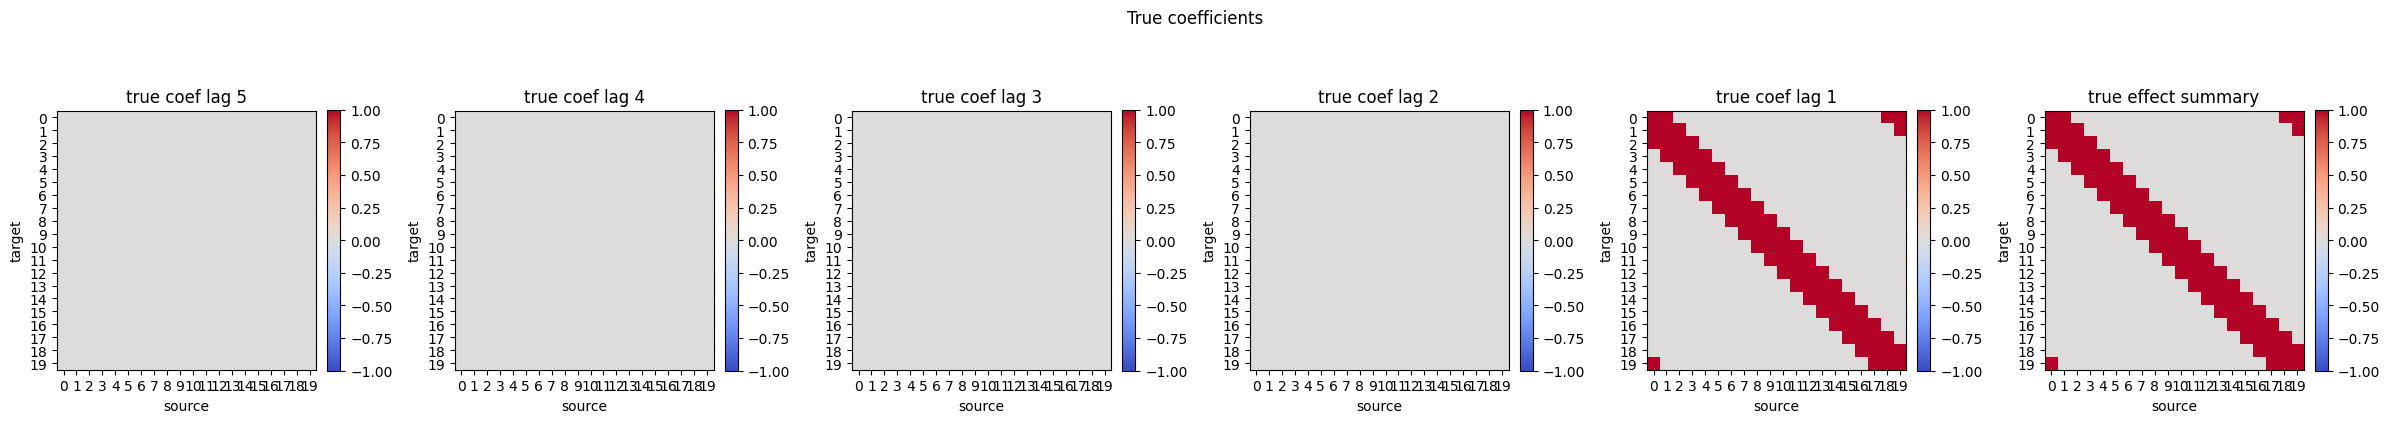
\includegraphics[width=0.9\linewidth]{lorenz96_true_graph.png}
\end{frame}


\begin{frame}{実験結果：推定精度}
\centering
\scriptsize
\textbf{表：各手法の最大性能}

\vspace{0.5em}

\setlength{\tabcolsep}{2.5pt}
\renewcommand{\arraystretch}{1.15}

\begin{tabular}{lcccc}
\toprule
手法
& \shortstack{線形VAR\\best F1}
& \shortstack{Lorenz-96\_1\\best F1}
& \shortstack{Lorenz-96\_2\\best F1}
& \shortstack{Lorenz-96\_2\\AUPRC} \\
\midrule

GSE-VAR
& \textbf{0.919} (SGL)
& \textbf{1.000} (HGL)
& \textbf{1.000} (HGL)
& \textbf{1.000} (HGL) \\

cMLP
& --
& 0.909
& 0.761
& 0.803 \\

GVAR
& --
& 0.909
& 0.793
& 0.903 \\

Linear VAR
& 0.878
& 0.775
& 0.620
& -- \\

\bottomrule
\end{tabular}
\center
Lorenz96\_1,Lorenz\_2はそれぞれ$(F=40,T=1000),(F=40,T=500)$の実験を表す。
\vspace{1.0em}
\begin{itemize}
  \item 3つの実験において、全ての手法を上回るスコア
  \item しかし、$\lambda_{ngc}$にF1が敏感。GVARも閾値に敏感。
  \item $\lambda_{ngc}$調整の手法の確立が最大の課題であるように感じた。
\end{itemize}
\end{frame}




\begin{frame}{Lorenz-96\_2：$\lambda_{ngc}$によるスコア推移(GSE-VAR)}
  \centering
  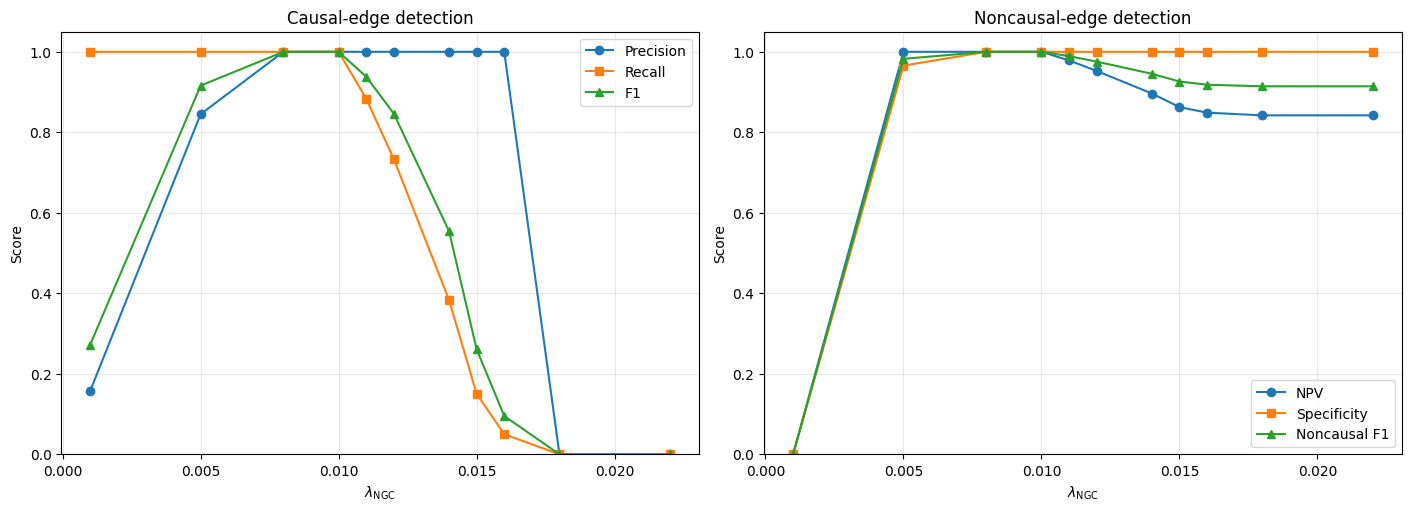
\includegraphics[width=0.95\linewidth]{scores_by_lambda.png}
\end{frame}

\begin{frame}{Lorenz-96\_2：$\lambda_{ngc}$によるPR曲線(GSE-VAR)}
  \centering
  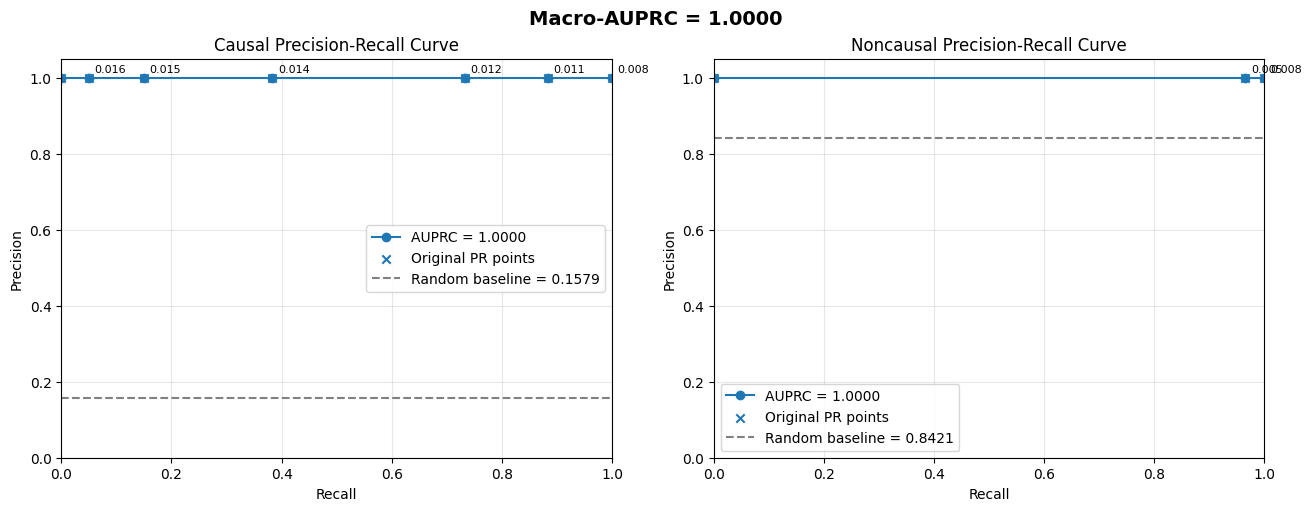
\includegraphics[width=0.90\linewidth]{PRcurve_ours.png}
\end{frame}

\begin{frame}{Lorenz-96\_2：$\lambda_{ngc}$によるPR曲線(cMLP)}
  \centering
  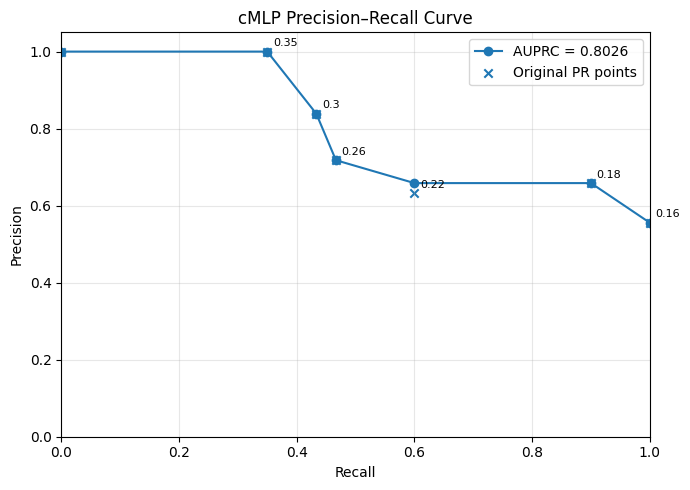
\includegraphics[width=0.90\linewidth]{PRcurve_cmlp.png}
\end{frame}

\begin{frame}{Lorenz-96\_2：$\lambda_{ngc}$によるPR曲線(GVAR)}
  \centering
  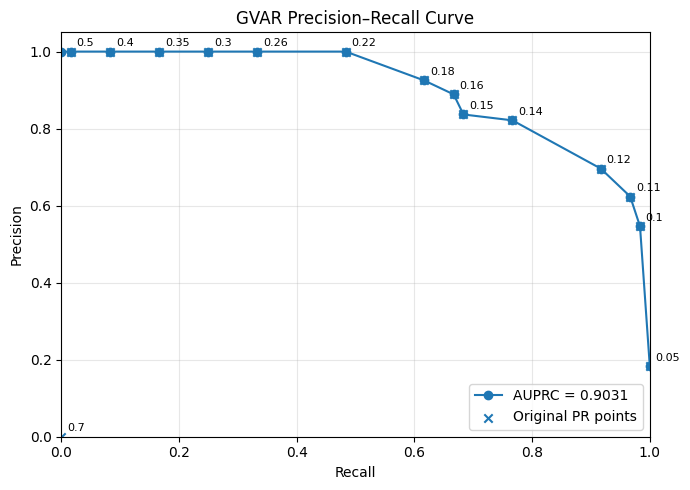
\includegraphics[width=0.90\linewidth]{PRcurve_gvar.png}
\end{frame}
\begin{frame}{Lorenz-96\_2：$\lambda_{ngc}$によるGranger因果行列}
  \centering
  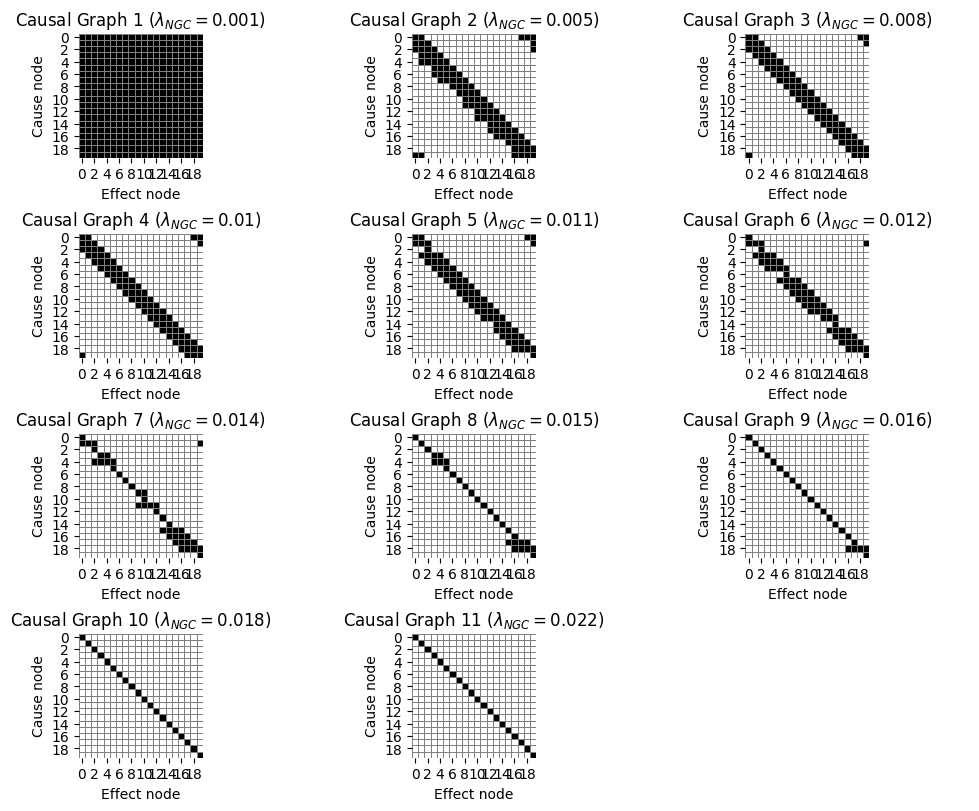
\includegraphics[width=0.7\linewidth]{causal_graph_by_lambda.png}
\end{frame}

\begin{frame}{線形データ：causal gate}
  \centering
  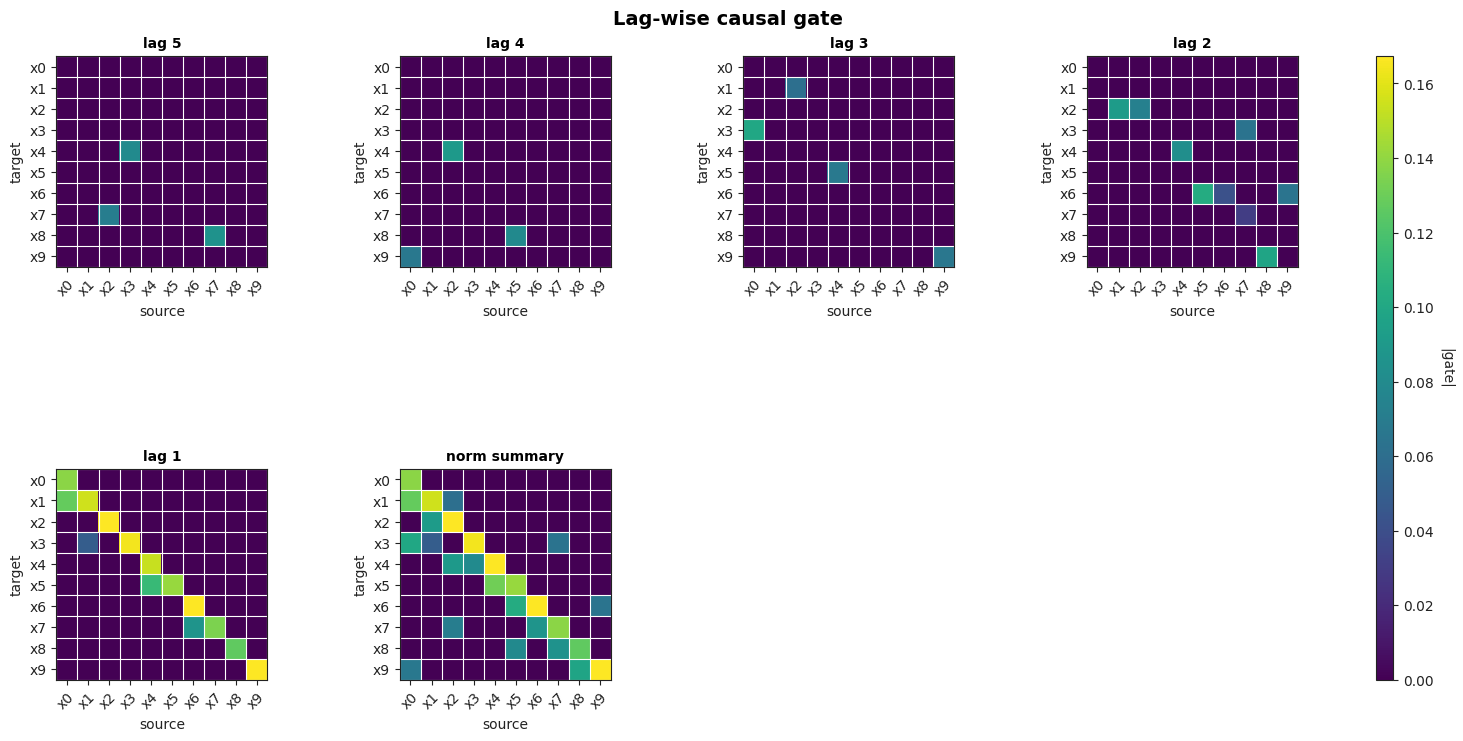
\includegraphics[width=0.8\linewidth]{linear_causal_gate.png}
    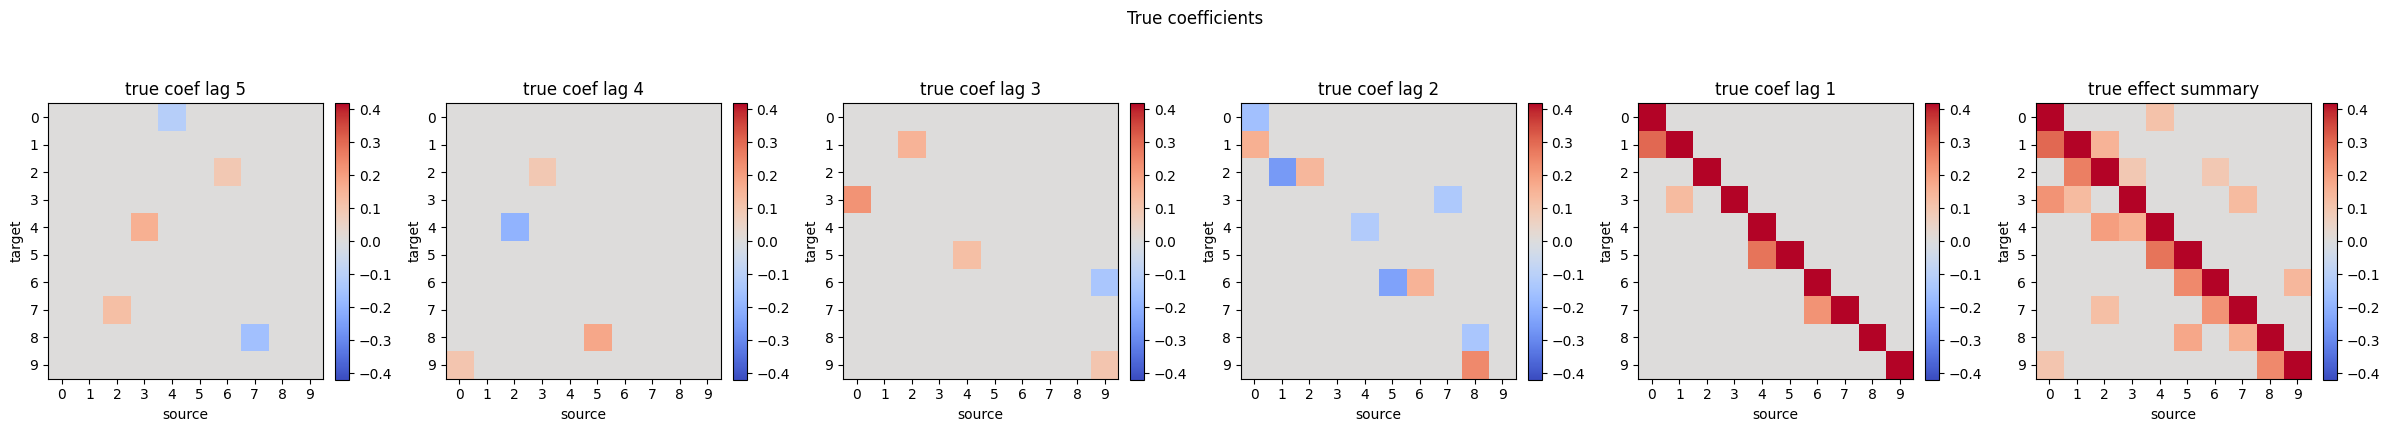
\includegraphics[width=1.0\linewidth]{linear_true_graph.png}
\end{frame}

\begin{frame}{線形データ：有効係数の符号確認}
  \centering
  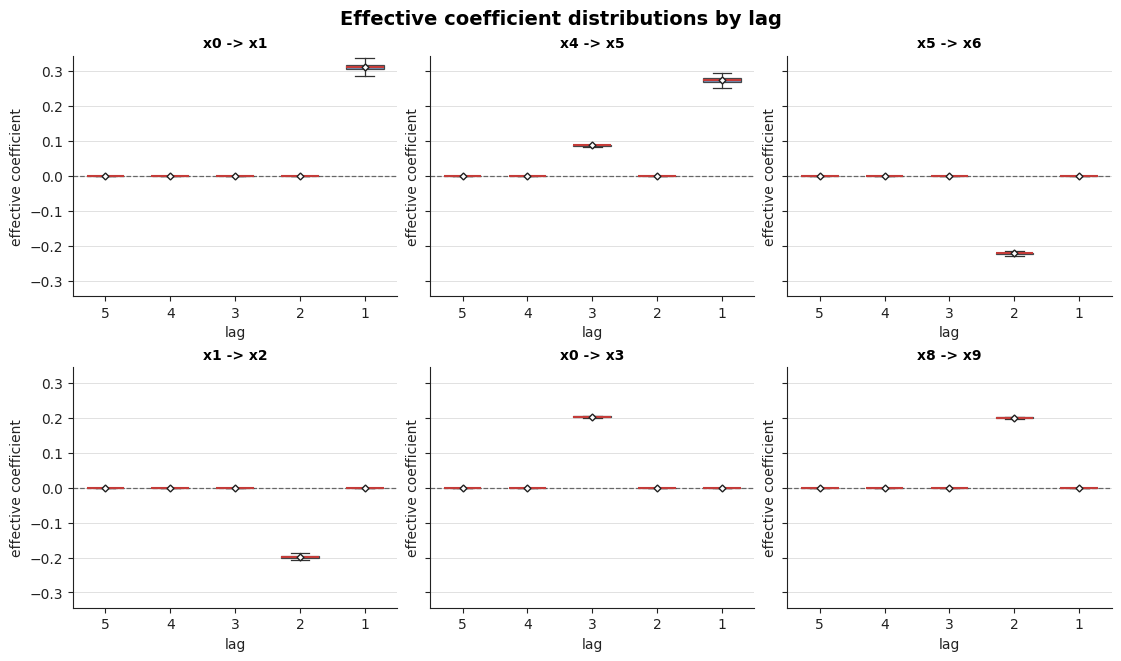
\includegraphics[width=0.95\linewidth]{linear_coef_boxplot.png}
\end{frame}

\begin{frame}{まとめ}
  \footnotesize
  本手法の要点は次の通りである。

  \begin{itemize}
    \item 入力値依存の係数による線形結合
    \item causal gateにより、入力依存の係数と静的なGranger因果構造を分離。
    \item causal gateに構造スパース化と近接勾配法を適用した。
  \end{itemize}

  \vspace{0.25em}
  これらの工夫により実現したのは、
  \begin{itemize}
    \item 高い表現力、解釈性
    \item 厳密にスパースなGranger因果行列を閾値無しで得ること
    \item 有効係数分布による効果の方向・強弱の確認
  \end{itemize}

  \vspace{0.25em}
  実験において、
  \begin{itemize}
    \item 線形データで係数の強度と符号のだいたいの一致を確認。
    \item 閾値無しでGranger非因果を推定できることを確認。
    \item ベンチマークにおいて全ての比較手法を上回るbestF1とAUPRCを達成。
  \end{itemize}
\end{frame}

\begin{frame}{今後の課題}
  本手法の課題は次の通りである。

  \begin{itemize}
    \item 最大精度の高さは示されたが、$\lambda_{\mathrm{ngc}}$によってエッジ数が急変するため、安定なチューニング方法の解明が必要。
    \item $pK$個の係数生成ネットワークを用いるため、スケーラビリティの問題がある。
    \item causal gateが正の実数範囲ある。ゲートを縮めてNN重みを拡大すれば、予測を変えずに罰則を小さくできてしまう。
  \end{itemize}
\end{frame}

\end{document}
